% %%%%%%%%%%%%%%%%%%%%%%%%%%%%%%%%%%%%%%%%%%%%%%%%%%%%%%%%%%%%%%%%%%%%%%%%%%%%%
% %%%%%%%%%%%%%%%%%%%%%%%%%%%%%%%%%%%%%%%% Survey of the Near-Earth Environment
% %%%%%%%%%%%%%%%%%%%%%%%%%%%%%%%%%%%%%%%%%%%%%%%%%%%%%%%%%%%%%%%%%%%%%%%%%%%%%

\chapter{From the Sun to the Earth}
\label{ch_intro}

It's all about energy transfer! 

Some example citations, including a few with special characters: \cite{dai_2013}, \cite{dai_2015}, \cite{lysak_2001}. 

%There are a lot of interrelated things going on, so it's hard to describe Earth's environment one step at a time. Look at Scott's thesis -- he did this well, right? 

%Heliosphere, Magnetosphere, Ionosphere, Atmosphere?

%Current systems, convective systems, density profiles? 

\begin{figure}
  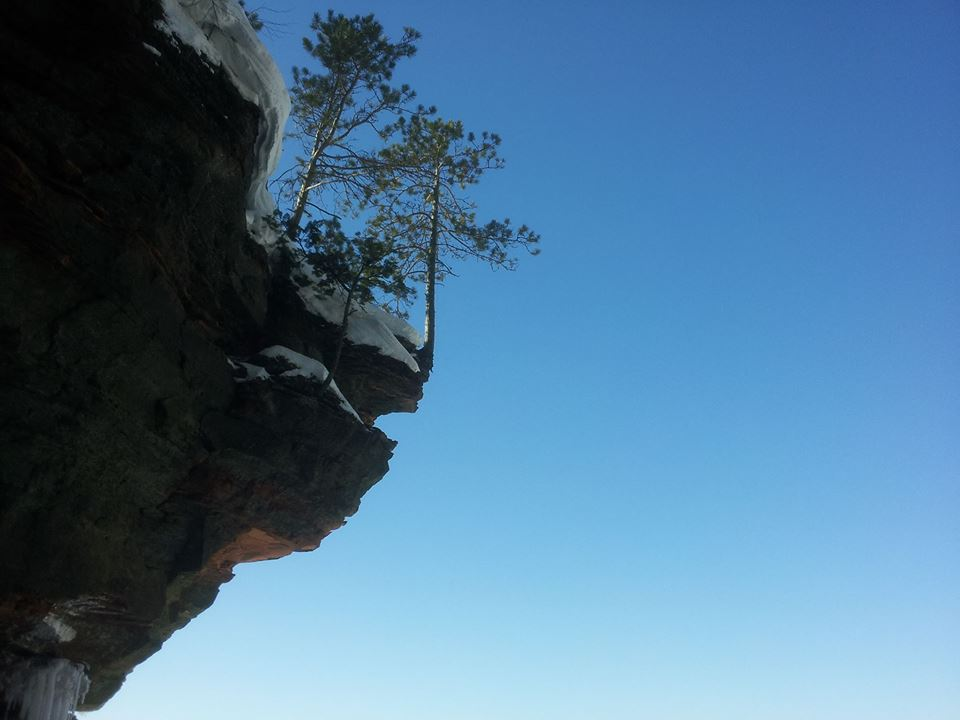
\includegraphics[width=5.75in, height=2in]{figures/image.jpg}
  \caption{Lorem ipsum dolor sit amet, consectetur adipiscing elit, sed do eiusmod tempor incididunt ut labore et dolore magna aliqua.}
  \label{fig_test}
\end{figure}

Sun generates energy through nuclear reactions. 

This energy drives behavior in the near-Earth environment. 

Typical solar wind density is $\sim \SI{5}{/\cm^3}$


\SI{45}{\degree} angle with the Earth-Sun line, which is the X direction. 
\footnote{We use uppercase $X$, $Y$, and $Z$ to indicate GSE coordinates: X points from the Earth to the Sun. Y is perpendicular to X, and in the Sun's ecliptic plane, pointing duskwards... against Earth's orbital motion. Points north, out of the ecliptic plane. Later, we will use lowercase $x$, $y$, and $z$ to define a more-or-less analogous corodinate system with respect to Earth.}

Solar wind is what deforms Earth's magnetic field to form the magnetosphere. 

Transient solar wind phenomena, such as coronal mass ejections, are also known to be related to geomagnetic disturbances at Earth. 





% =============================================================================
% =============================================================================
% =============================================================================
\section{The Outer Magnetosphere}

\subsection{The Magnetopause}

\subsection{The Magnetotail}

\subsection{Cusp Regions}

% =============================================================================
% =============================================================================
% =============================================================================
\section{The Inner Magnetosphere}

Characteristic profiles for $\omega_P$, $\Omega$, $v_A$, $\sigma$, $\epsilon$...

Table: bounce times as a function of L. How much does this depend on day vs night, storm vs calm? 

\subsection{The Plasmasphere}

\subsection{Ring Currents}

\subsection{The Radiation Belts}

% =============================================================================
% =============================================================================
% =============================================================================
\section{Geomagnetic Disturbances}

\subsection{Storms}

\subsection{Substorms}






